\label{sec:framework}

This section presents the ontology construction process and its integration into the retrieval pipeline. Section~\ref{ssec:formal} gives formal definitions. Section~\ref{ssec:hierarchy} describes the ingredient hierarchy and dish taxonomy. Section~\ref{ssec:relations} details relation derivation. Section~\ref{ssec:integration} explains the two ontology injection points.

% ──────────────────────────────────────────────────────────────
\subsection{Formal Definition}
\label{ssec:formal}

We define the food ontology as a tuple $\mathcal{O} = (\mathcal{C}, \mathcal{R}, \mathcal{I}, \mathcal{A})$, where $\mathcal{C}$ is a set of classes organized in a rooted tree (T-box - Fig.~\ref{fig:hierarchy}), $\mathcal{R}$ is a set of named relation types, $\mathcal{I}$ is a set of instances (ingredients and dishes), and $\mathcal{A}$ is a set of assertions linking instances to classes and to each other (A-box - Fig.~\ref{fig:abox-bunbohue}). The class hierarchy supports the \emph{subClassOf} relation: if $c_1 \sqsubseteq c_2$, then every instance of $c_1$ is also an instance of $c_2$. Table~\ref{tab:relations} lists the six named relations with their derivation sources and corpus-level counts.

\begin{table}[t]
\centering
\caption{Named relations in the food ontology.}
\label{tab:relations}
\small
\begin{tabular}{llll}
\toprule
\textbf{Relation} & \textbf{Signature} & \textbf{Derivation} & \textbf{Count} \\
\midrule
hasIngredient      & dish $\times$ ing            & direct from KB     & 10{,}741 \\
mainIngredient     & dish $\times$ ing            & importance $\geq$ 3 & 10{,}741 \\
subClassOf         & class $\times$ class         & manual curation    & 48 \\
flavorComplements  & ing $\times$ ing             & NPMI $>$ 0.3      & 15{,}119 \\
conflictsWith      & ing $\times$ ing             & curated rules      & 139 \\
cookedBy           & dish $\times$ method         & category pattern   & 10{,}741 \\
\bottomrule
\end{tabular}
\vspace{2pt}
  \par\noindent\footnotesize\textit{Note:} ing = ingredient; KB = knowledge base.
\end{table}

\begin{figure}[t]
\centering
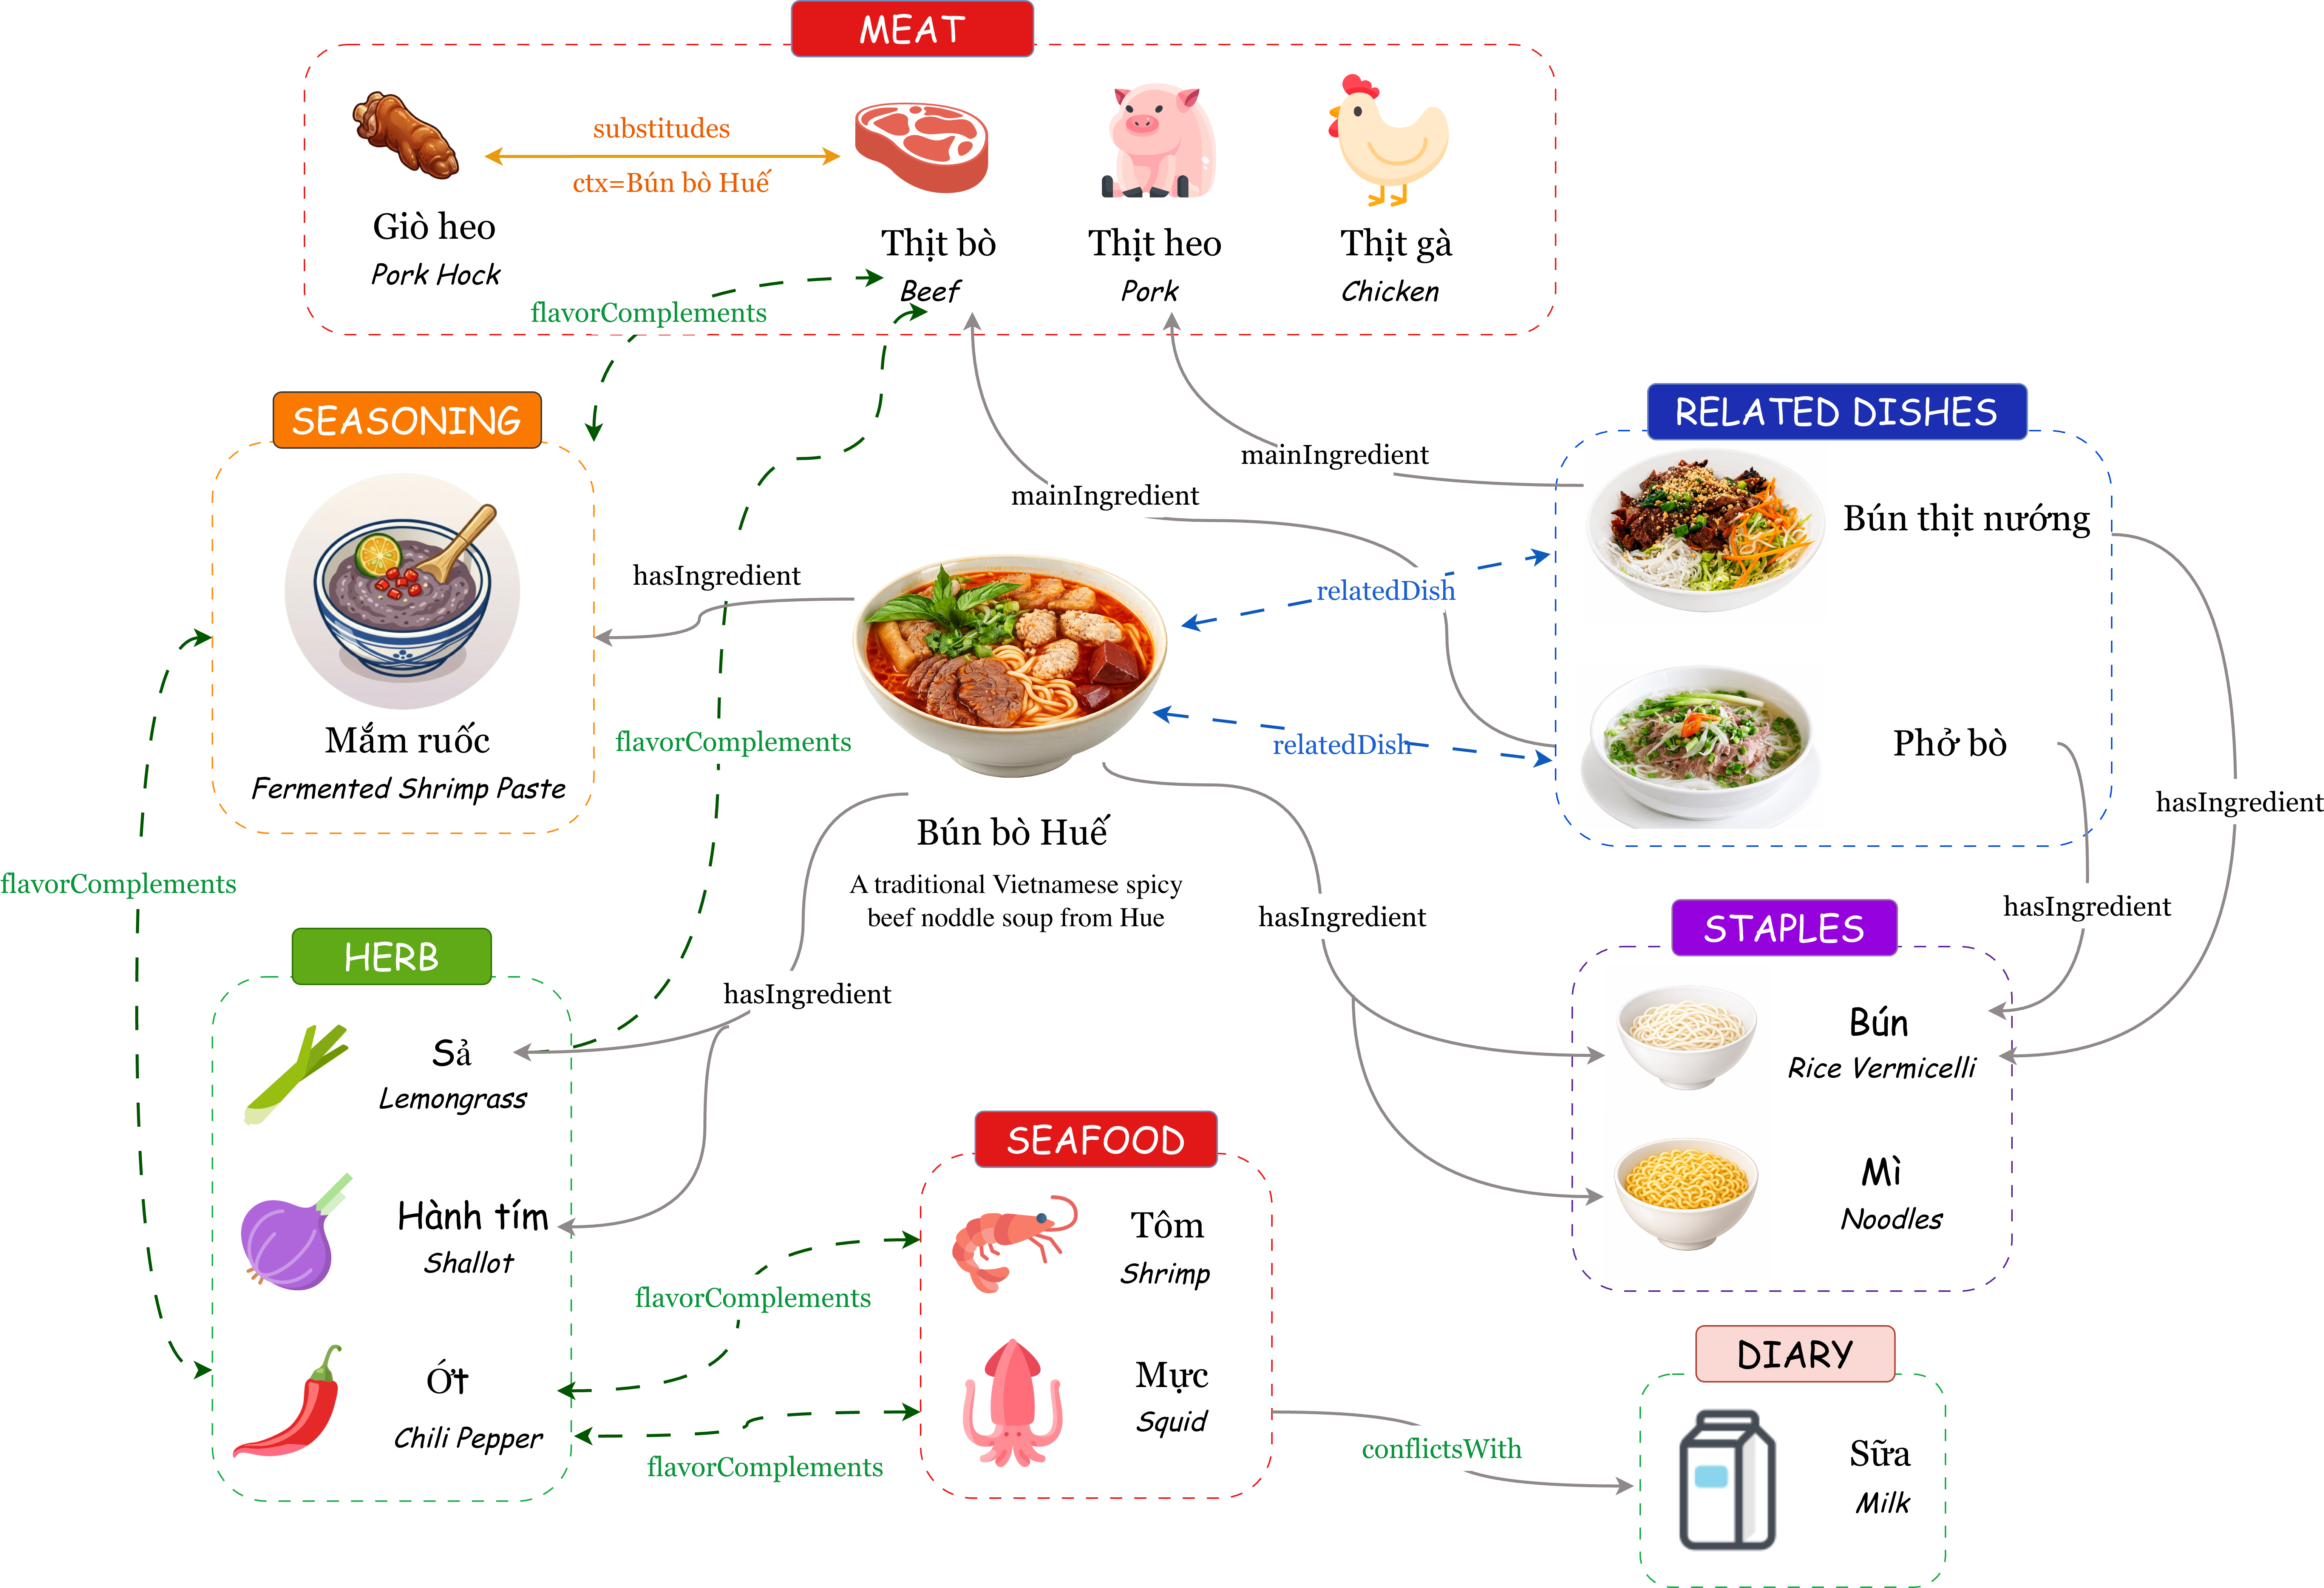
\includegraphics[width=\columnwidth]{figures/a-box.png}
\caption{Illustrative A-box example of instance-level relations in the Vietnamese food ontology.}
\label{fig:abox-bunbohue}
\end{figure}

% ──────────────────────────────────────────────────────────────
\subsection{Ingredient Hierarchy and Dish Taxonomy}
\label{ssec:hierarchy}

\textbf{Ingredient hierarchy.}
The ingredient hierarchy is a four-level rooted tree with 49 classes (24 leaf classes) covering 2{,}112 Vietnamese ingredients. Level~0 is the root \texttt{Ingredient}; Level~1 contains nine top categories (\texttt{Protein}, \texttt{Produce}, \texttt{Seasoning}, \texttt{Staple}, \texttt{Dairy}, \texttt{Beverage}, \texttt{Sweet}, \texttt{Processed}, \texttt{Other}); Level~2 and Level~3 provide finer distinctions (e.g., \texttt{Protein} $\to$ \texttt{AnimalProtein} $\to$ \texttt{Seafood}). Construction follows a two-stage process: (1)~manual design of the class tree based on Vietnamese culinary conventions, and (2)~automated classification of each ingredient into a leaf class using an LLM classifier (Qwen-2.5 7B, temperature~0, batch size~25), with manual validation of the 100 most frequent ingredients and spot-checking of 50 random samples. Ingredients that cannot be resolved are assigned to a fallback \texttt{Other} class. Fig.~\ref{fig:hierarchy} illustrates the top three levels.

\begin{figure}[t]
\centering
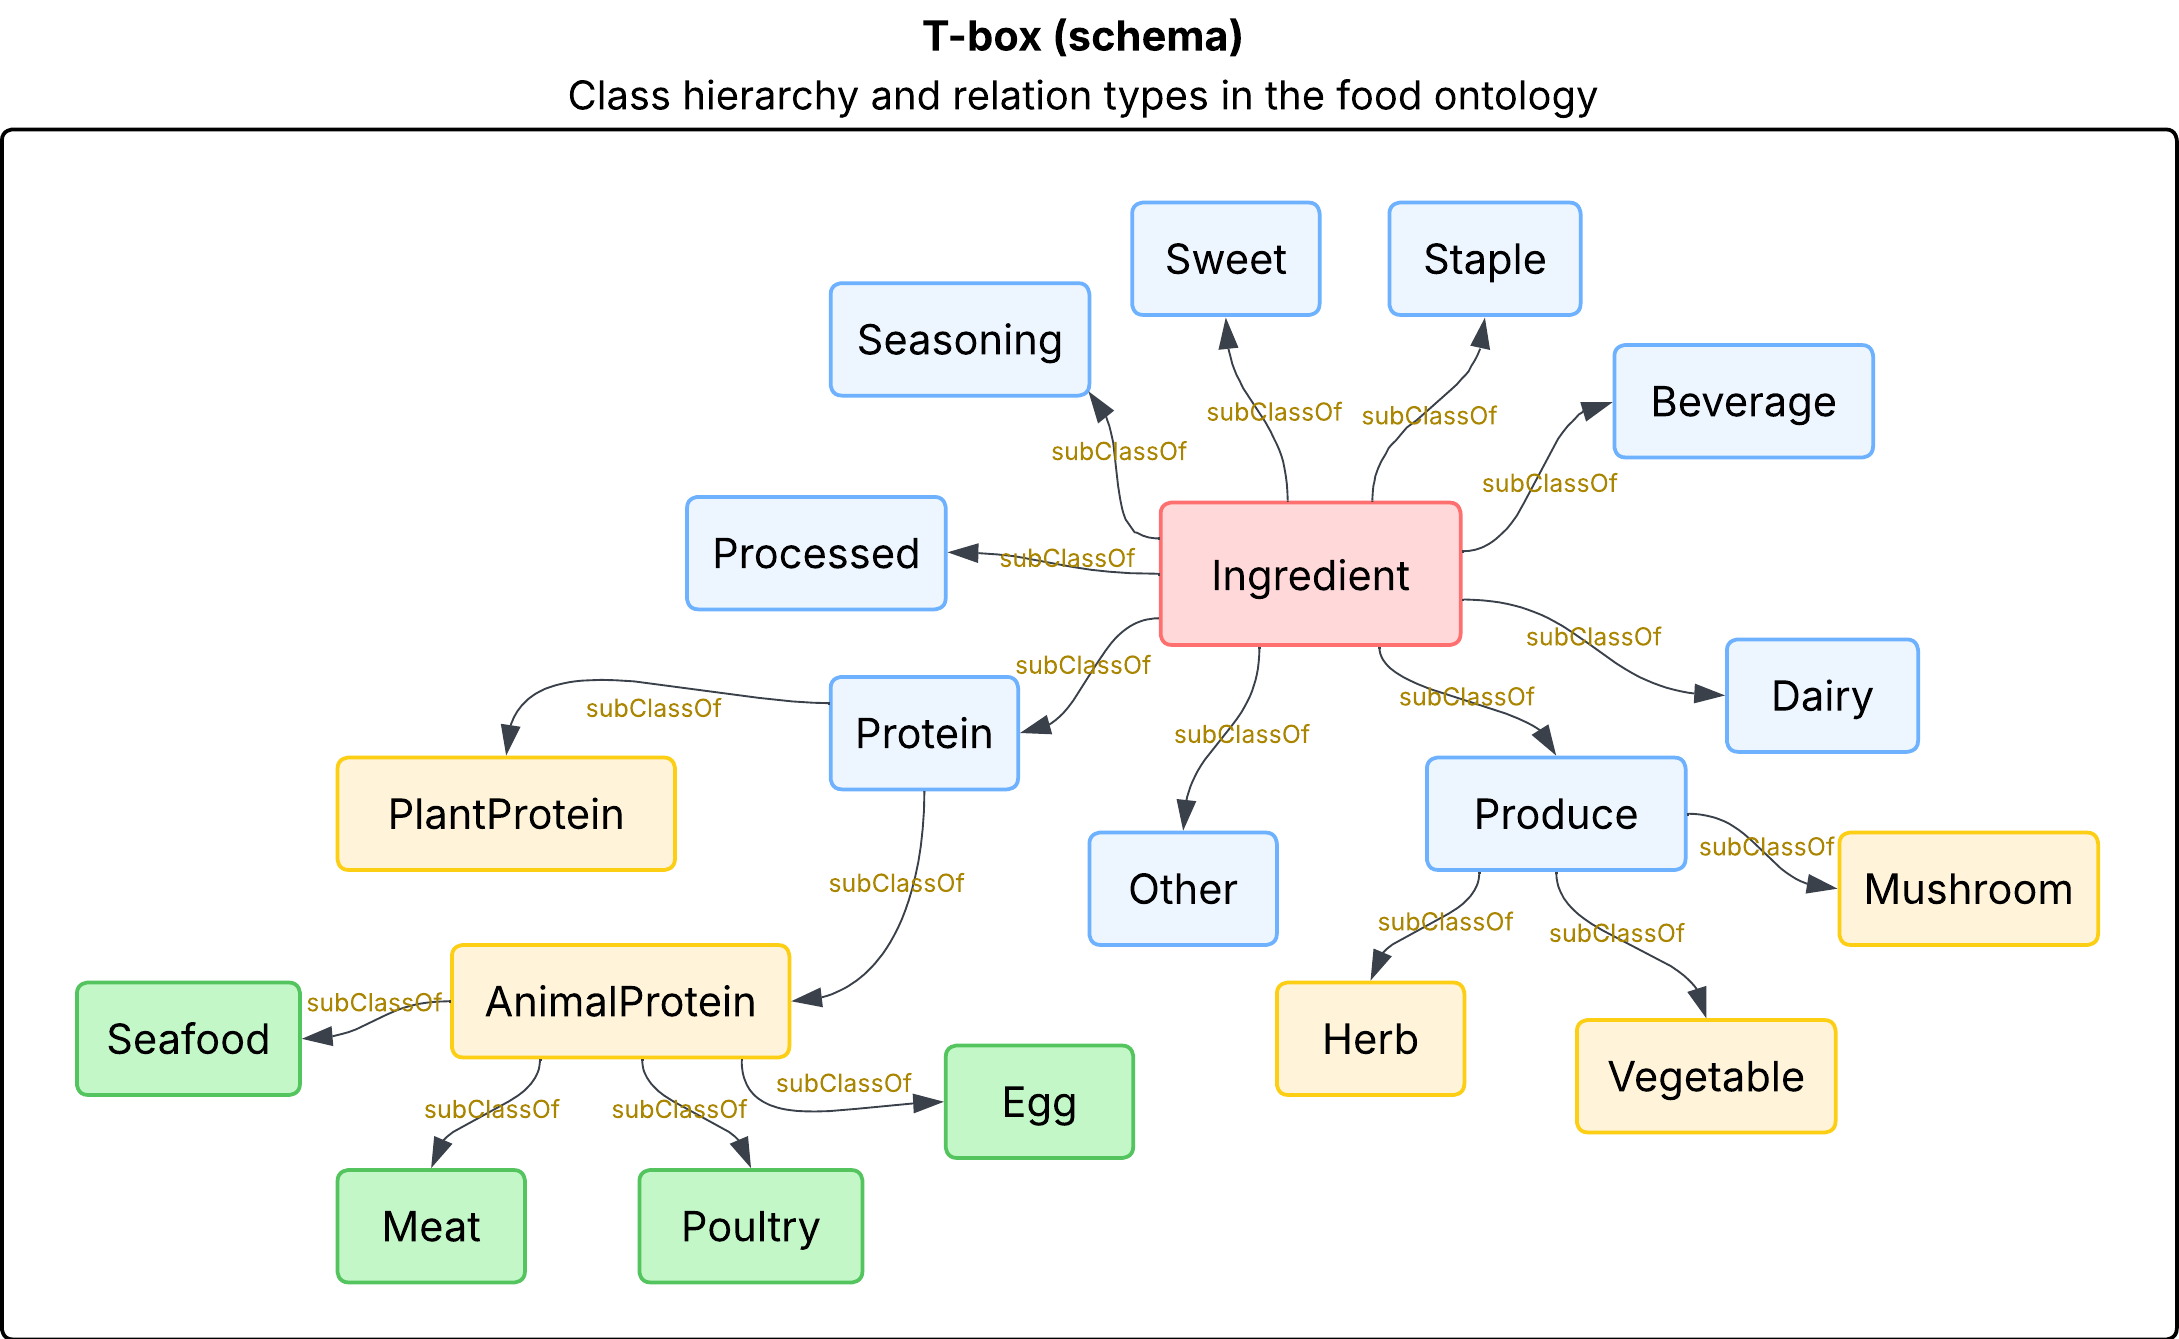
\includegraphics[width=\columnwidth]{figures/hierarchy_tree.png}
\caption{Class hierarchy of the Vietnamese food ontology. Only subClassOf relations are shown; the six named relations between instances are listed in Table \ref{tab:relations}.}
\label{fig:hierarchy}
\end{figure}

\textbf{Dish taxonomy.}
Dishes are classified along two orthogonal axes. The \emph{byType} axis groups dishes into 25 culinary categories (e.g., \texttt{mon\_canh}, \texttt{mon\_kho}, \texttt{mon\_xao}, \texttt{mon\_nuong}). The \emph{byMethod} axis maps each category to one of 24 cooking-method labels (e.g., \texttt{Boil}, \texttt{Stew}, \texttt{StirFry}, \texttt{Grill}), derived from the dish category field via pattern matching. All 10{,}741 dishes receive a cooking-method assignment.

% ──────────────────────────────────────────────────────────────
\subsection{Relation Derivation}
\label{ssec:relations}

Each relation is derived from existing data artifacts rather than manual annotation.

\textbf{flavorComplements($A$, $B$).}
We compute Normalized Pointwise Mutual Information (NPMI)~\cite{bouma2009npmi} over ingredient co-occurrence across all 10{,}741 dishes:
%
\begin{equation}
\label{eq:npmi}
\text{NPMI}(A, B) = \frac{\log \frac{P(A, B)}{P(A)\,P(B)}}{-\log P(A, B)}
\end{equation}
%
where $P(A,B)$ is the joint co-occurrence probability of ingredients $A$ and $B$, and $P(A)$, $P(B)$ are their marginal probabilities estimated from dish co-occurrence counts. All pairs with $\text{NPMI} > 0.3$ are retained, yielding 15{,}119 complement pairs.

\textbf{conflictsWith($A$, $B$).}
139 nutritional and medical conflict rules are imported from an existing curated conflict database and normalized to ontology ingredient identifiers. While not used directly in the dish similarity formula (as ingredient conflicts within a single dish do not indicate dissimilarity between two dishes), this relation supports downstream applications such as meal planning and recipe safety validation.

\textbf{cookedBy(dish, method).}
The cooking method is mapped from the dish category field using a 25-entry lookup table (e.g., ``m\'{o}n x\`{a}o'' $\to$ \texttt{StirFry}), covering all 10{,}741 dishes.

% ──────────────────────────────────────────────────────────────
\subsection{Ontology Integration with Dense Retrieval}
\label{ssec:integration}

The ontology is injected into the dense-retrieval pipeline at two points, each targeting one of the failure modes identified in Section~\ref{sec:introduction}. Fig.~\ref{fig:pipeline} illustrates the overall architecture.

\begin{figure}[!htbp]
  \centering
  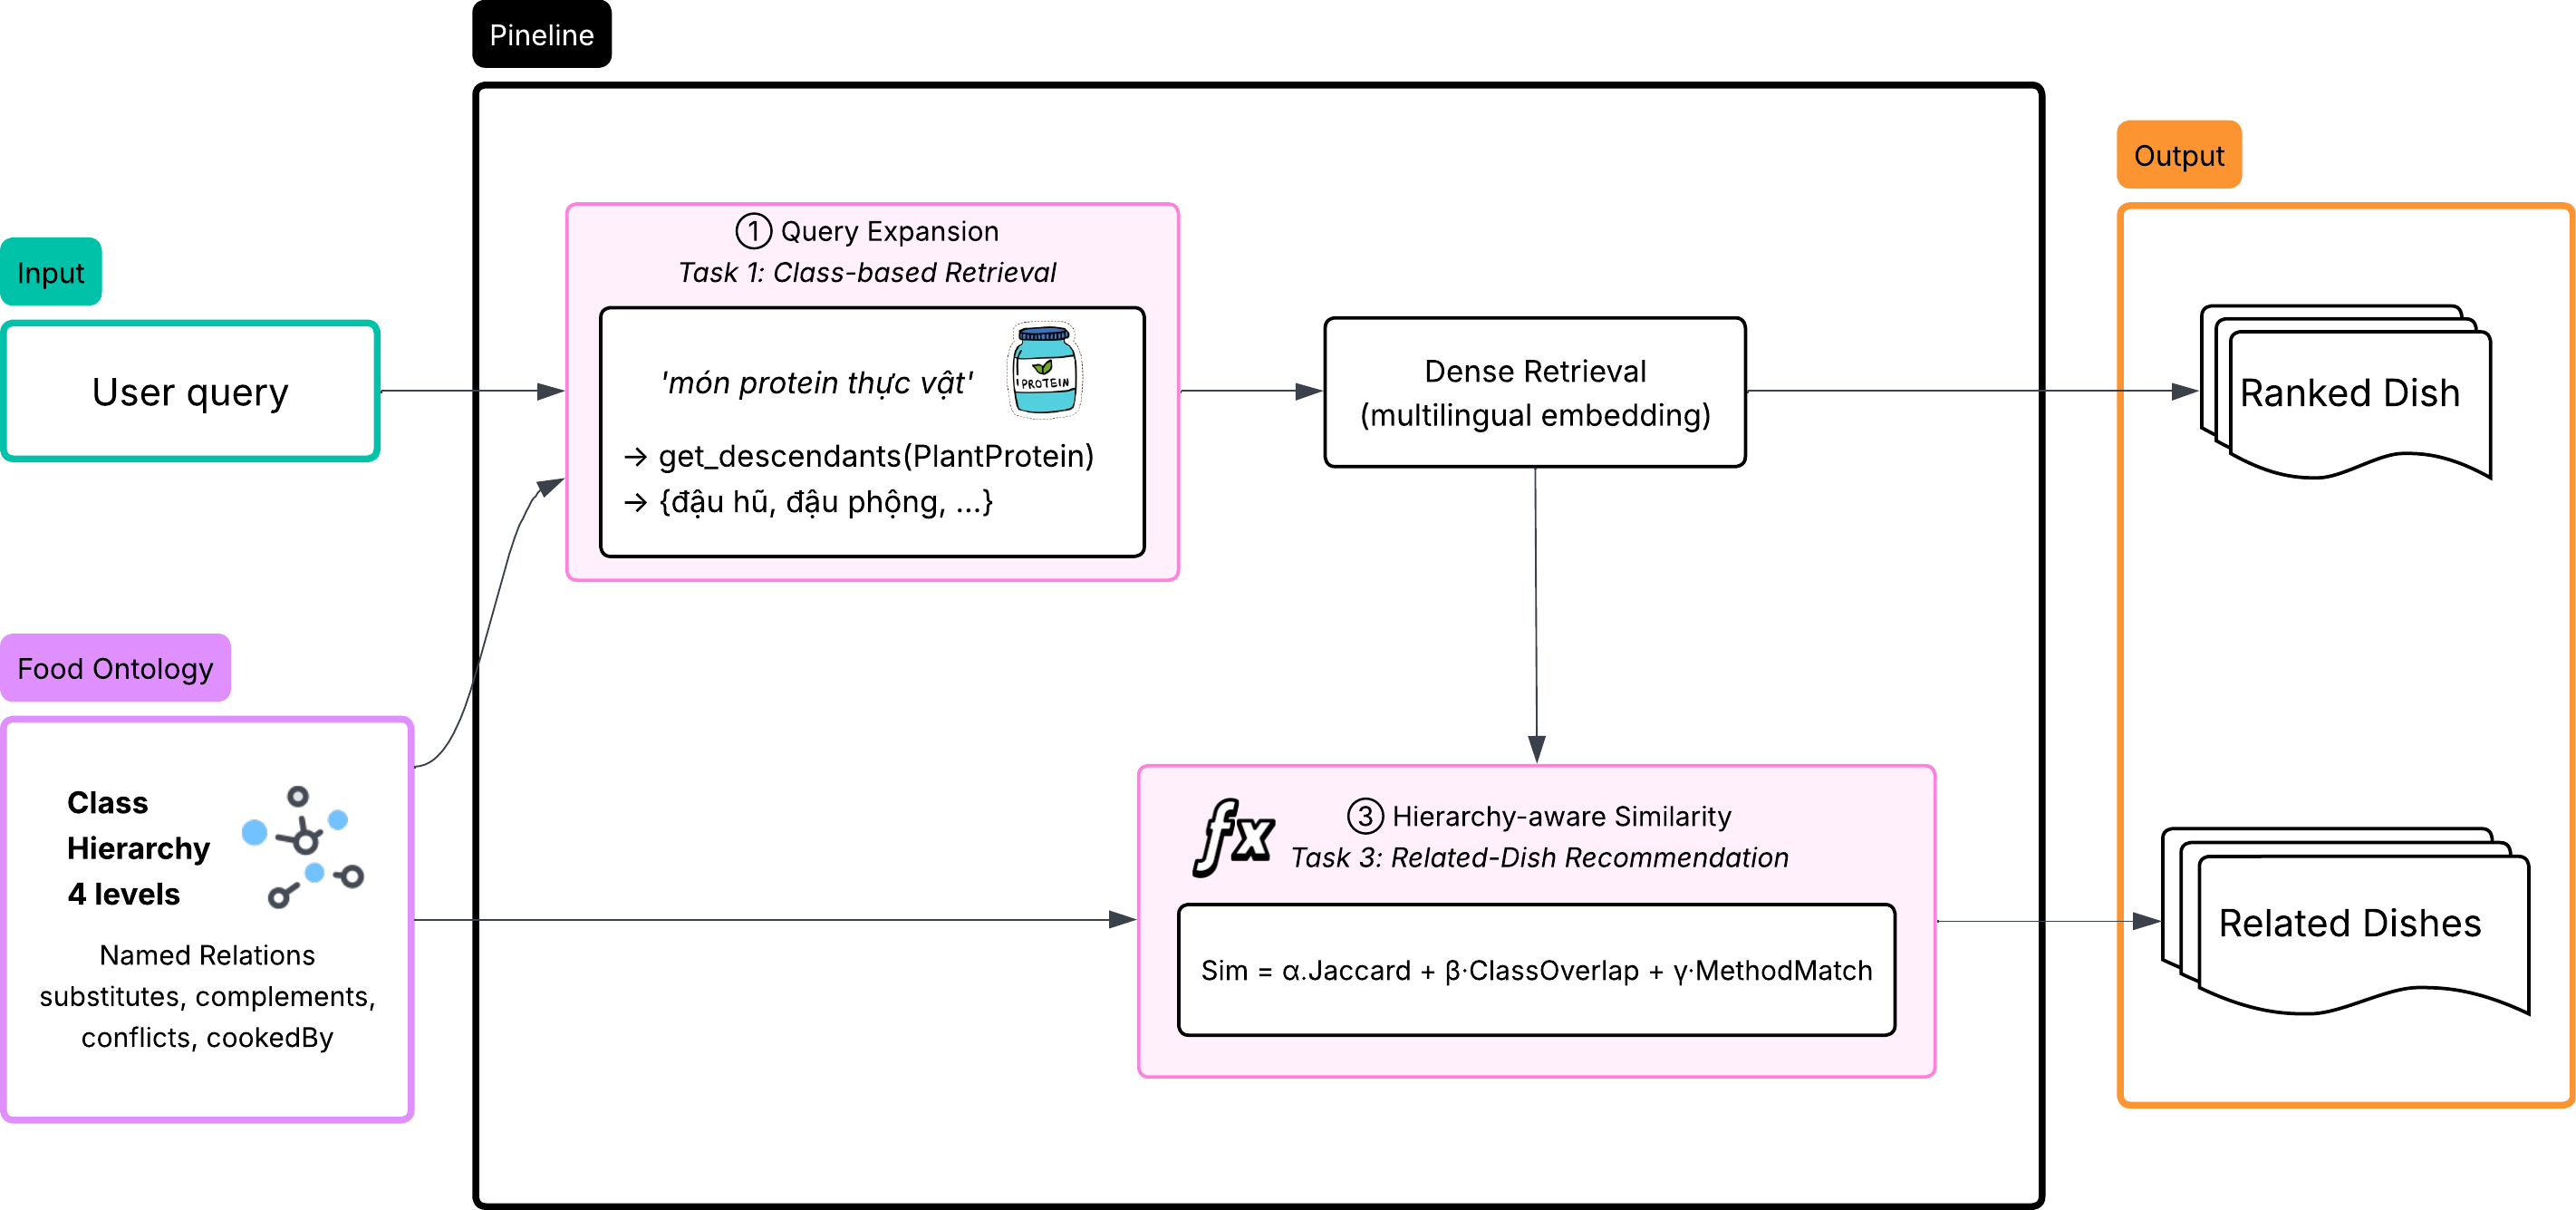
\includegraphics[width=\linewidth]{figures/pipeline.png}
  \caption{Ontology injection points in the retrieval pipeline.}
  \label{fig:pipeline}
\end{figure}

\textbf{(1) Query expansion (Task~1).}
For class-level queries such as \textit{món protein thực vật}
(plant-protein dishes), the system maps the class term to an ontology node and retrieves all descendant ingredient names. The expanded ingredient list is appended to the original query before dense encoding. Negation queries (e.g., \textit{món không hải sản}
(dishes without seafood)) expand the positive class and exclude matching dishes at retrieval time.

\textbf{(2) Hierarchy-aware dish similarity (Task~2).}
Dish similarity combines five components:
%
\begin{equation}
\label{eq:sim}
\text{Sim}(A, B) = \alpha \cdot J + \beta \cdot C + \gamma \cdot M + \delta \cdot S + \varepsilon \cdot F
\end{equation}
%
where $A$ and $B$ are two dishes represented by their ingredient sets, and $\alpha, \beta, \gamma, \delta, \varepsilon$ are tunable weights (summing to 1.0) determined via 5-fold cross-validation (Section~\ref{ssec:eval_protocol}). 

These five components are specifically chosen to capture the multifaceted nature of culinary similarity, moving beyond simple keyword matching. Exact ingredient overlap ($J$) provides a foundational baseline, while class overlap ($C$) accounts for valid within-category substitutions (e.g., swapping two types of animal protein). Cooking method ($M$) is critical because identical ingredients can yield entirely different dishes when boiled versus grilled. Finally, semantic similarity ($S$) and flavor complementarity ($F$) are incorporated to capture nuanced contextual relationships and traditional gastronomic pairings (e.g., ginger and seafood). The five components are mathematically defined as follows:

\begin{itemize}
  \item $J = \text{WeightedJaccard}(A, B)$: Ingredient overlap weighted by role importance. Each ingredient $i$ receives a weight $w_i \in \{3.0, 1.5, 0.5\}$ for main, secondary, and seasoning roles respectively. These precise weights were empirically determined through preliminary trials to maximize retrieval performance, effectively reflecting the decreasing semantic importance of ingredients based on their specific culinary roles.
  \[
    J = \frac{\sum_{i \in A \cap B} w_i}{\sum_{i \in A \cup B} w_i}
  \]

  \item $C = \text{WeightedClassOverlap}(A, B)$: Greedy bipartite matching over ontology classes. Each matched pair scores 1.0 (same leaf class) or 0.5 (same parent class), multiplied by the ingredient's role weight $w_i$, and normalized by the total weight:
  \[
    C = \frac{\sum_{a \in A} w_a \cdot \text{match}(a, B)}{\sum_{a \in A} w_a}
  \]
  These specific scoring assignment thresholds (1.0 and 0.5) were selected as the optimal configuration after multiple experimental iterations to effectively reward close taxonomic proximity while appropriately penalizing broader, distant parent-class matches.

  \item $M = \text{MethodMatch}(A, B)$: Returns 1.0 if both dishes share the same cooking method (e.g., both stir-fried), 0.0 otherwise.

  \item $S = \text{SemanticSim}(A, B)$: Mean pairwise semantic similarity between ingredients of $A$ and $B$, computed from pre-trained embedding matrices.

  \item $F = \text{FlavorComplement}(A, B)$: Mean NPMI of cross-dish ingredient pairs that appear as \texttt{flavorComplements} in the ontology. Captures flavor affinity: dishes sharing complementary flavor profiles (e.g., ginger--seafood, lemongrass--beef) receive higher scores. Returns 0 if no complement pairs exist between the two dishes.
\end{itemize}